\documentclass[11pt]{book}
\usepackage{palatino}
\usepackage{amsfonts,amsmath,amssymb}
\usepackage{pdfpages}
\usepackage{tikz}
\usepackage{geometry} % Keep the original margins
\usepackage{subcaption} % Add the subcaption package
\usepackage{booktabs}
\usepackage{graphicx}
\usepackage{epstopdf}
\usepackage{accents}
\usepackage{adjustbox} % For vertical alignment

\begin{document}
\pagestyle{empty}
{\noindent\bf Summer C 2024 \hfill Alexis  G.L.~Leclerc}
\vskip 16pt
\centerline{\bf University of Central Florida}
\centerline{\bf Department of Economics}
\vskip 16pt
\centerline{\bf ECO 4934}
\centerline{\bf Topics in Econometrics}
\vskip 10pt
\centerline{\bf Group B - Week 2 - Memo}
\vskip 32pt
\noindent

This week we will split the dataset into Train-Test-Validation datasets and complete the code for the logit/logit-lasso model. Additionally we will begin the HTML code.
\begin{center}Tasks completed (up to 07/08/2024):\end{center}
\begin{itemize}
    \item[1.] Created Github Repository and Codespace for the project. 
    \item[2.] Cleaned CSV files. Using primary keys~~ id,~~`who`,~~`when`.
    \item[3.] Created MySQL DB along with tables for each CSV file. 
    \item[4.] Joined tables to reports using LEFT JOIN by primary keys, Exported table to .dat\vspace{\baselineskip}
\vspace{\baselineskip}

   \hspace{2em} ER Diagram on 2nd page.
\end{itemize}
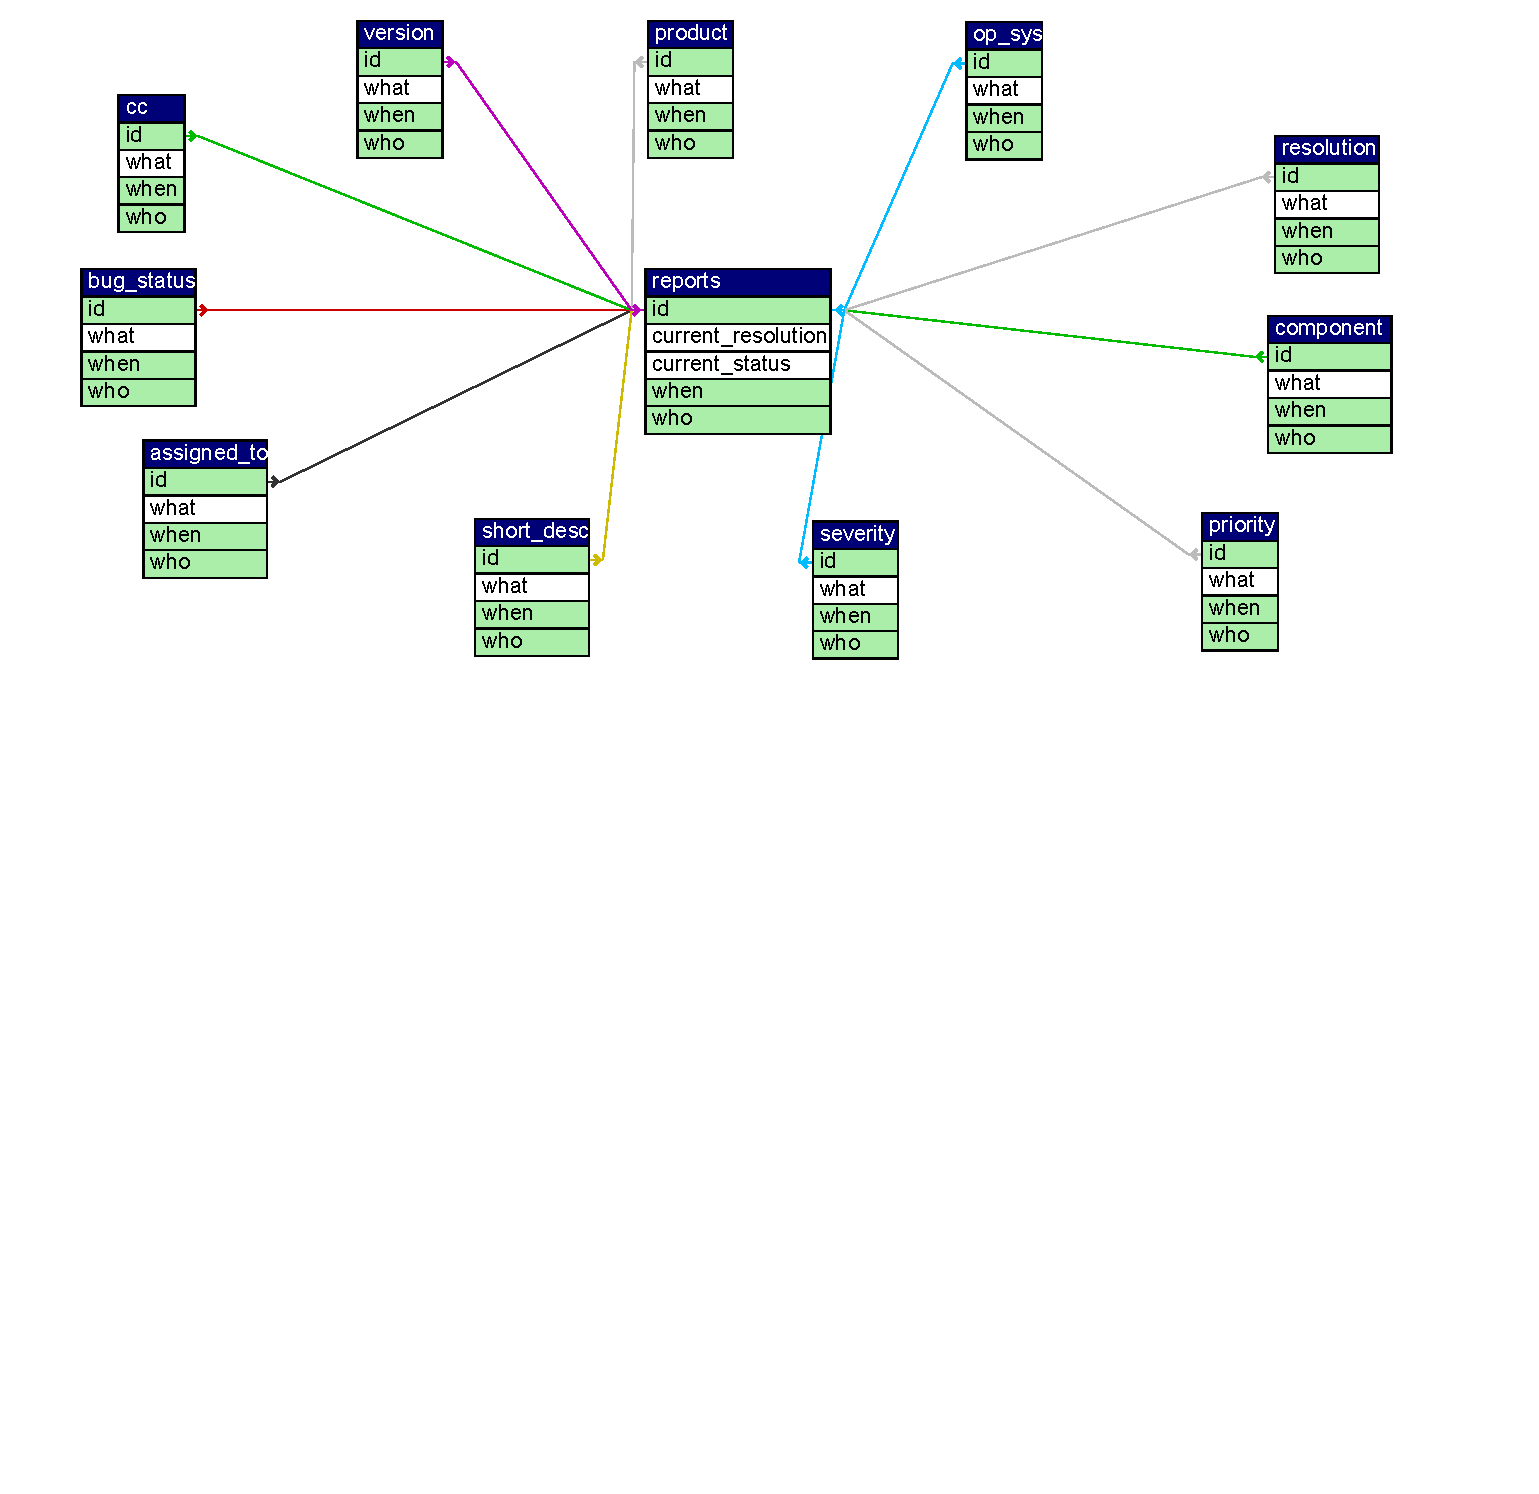
\includepdf[pages=-]{MEMOS/Week2/ER_D.pdf}

\end{document}
